\section{SiPM Simulation}

In addition to studying the new electronics with the test beam, we also did a SiPM simulation which could use theoretical signal from the detector and give the SiPMs response to them. When the light from the detector goes to the SiPM a Y11 light mixer is used so that the light is spread across the pixel face. The light mixer has a unique shape in which is shines the light onto the pixel face. Using a mathematical representation of this pulse shape we can simulate how light is shined on the pixel face. We can then create a virtual pixel face that has accurate geometric representation of the pixel face. Each of these virtual pixels could be activated by the incoming Y11 light pulse and would respond by firing off a set amount of charge just like an actual SiPM would. When these pixels are activated they also have a certain probability to activate a neighboring pixel which will simulate the cross talk of the SiPM. Each pixel also has a recharge rate so if it is hit in rapid succession it will fire with a reduced amount of charge emulating the saturation effect. Using this simulation we easily adjust the number of input photons and get very good details of the SiPM response. We can also easily turn different things off to see how significant individual effects are. This simulation is capable of producing more fine tuned data and in greater quantities than test beam data. In addition, it is able to simulate situations that are not possible in the test beam. On the other hand the accuracy of this simulation is heavily dependent on the data we input into it.

Since the program can simulate the non-linearity effects of the SiPM, we can use theoretical inputs to the SiPM to study its effects. The light a particle deposits in a scintillator tile can vary in time the Y11 light mixer ensures that the input light pulse shape remains constant. This means to change energy of the incident particle we just have to increase the number of photons in the input pulse while keeping the same shape. The output of the virtual SiPM is normalized so if the simulation was a completely linear device its output "charge" should exactly equal the number of input photons. 

\begin{figure}
\centering
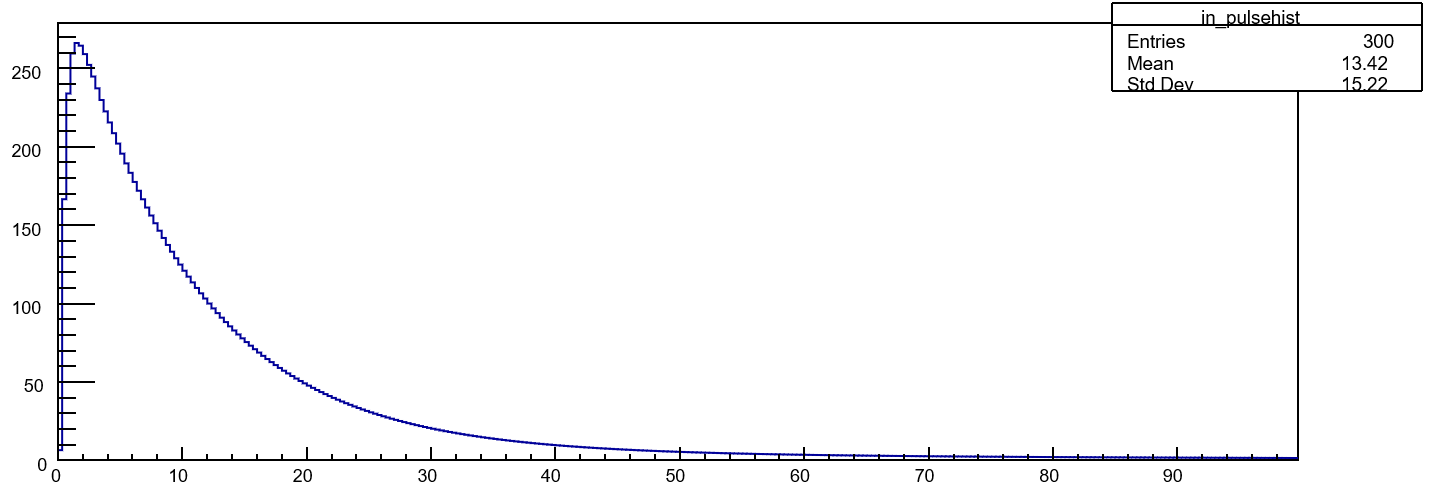
\includegraphics[width=\linewidth]{Figures/Y11.png}
\caption{A graph of the Y11 pulse shape with nanoseconds on the x axis and number of incident photons on the y axis}
\label{fig:Y11}
\end{figure}

\section{Simulation Analysis}

To do the analysis using the SiPM simulation, we simply measure the total output of the SiPM over a light pulse and compare it to the number of input photons. Since there is a degree of randomness we will use the average pulse over several inputs. Compared to using test beam data the analysis with the simulation is simple. In test beam the energy of the particle is spread over several SiPMs while in the simulation we have a very fine control of the input energy to the single SiPM. With a plot of input number of photons vs SiPM output charge we then create a correction curve that is necessary to make the graph linear. This is process for doing a non-linearity analysis using test beam data so we can compare the two correction curves to see if there is agreement. With other analyses it is common to simply divide out the cross talk. Given that there is a $15.4\%$ chance of crosstalk with a large signal of several thousand photons it is assumed that $15.4\%$ of the signal from the SiPM is due to cross talk so that number is simply divided out. This means the majority of the effects that the correction curve is compensating for is saturation. 

\begin{figure}
\centering
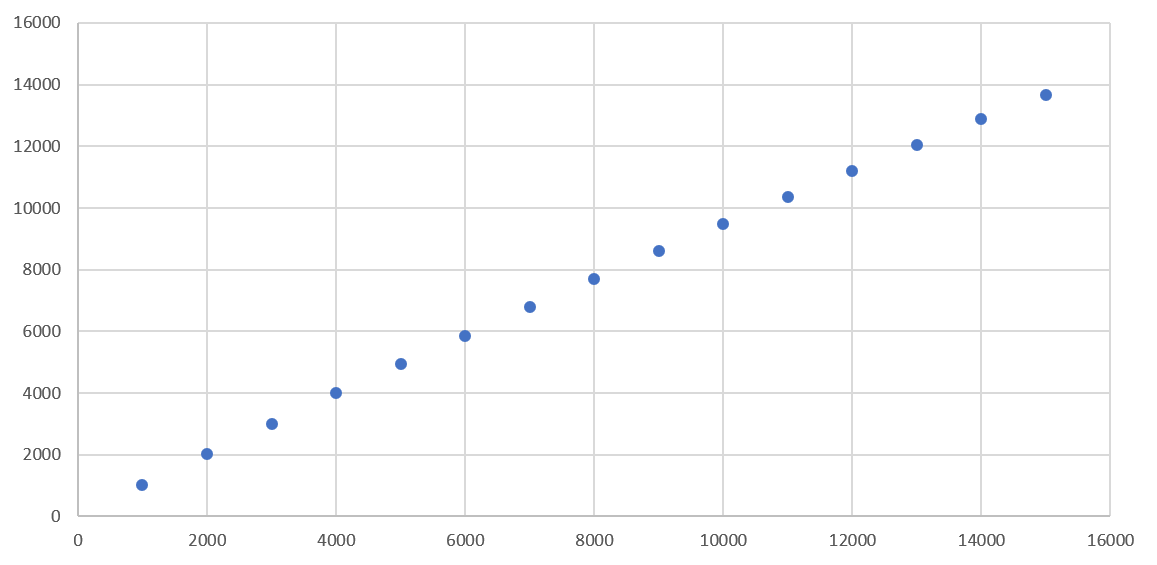
\includegraphics[width=\linewidth]{Figures/SimNon.png}
\caption{Graph of number of incident photons vs output charge of the SiPM simulation. Given the units of the simulation a perfectly linear device would have all data points falling on the y=x line but as shown as the number of incident photons is increased the data points fall short of this line.}
\label{fig:SimNon}
\end{figure}

To be sure the simulation is designed correctly it is useful to compare things like non-linearity to the actualy SiPM. Figure~\ref{fig:NonLin} shows the non-linearity of the SiPM from shining a laser directly on the SiPM. Figure~\ref{fig:Cor} shows a similar plot constructed using the simulation. There is significant disagreement between these two sets of data.

\begin{figure}
\centering
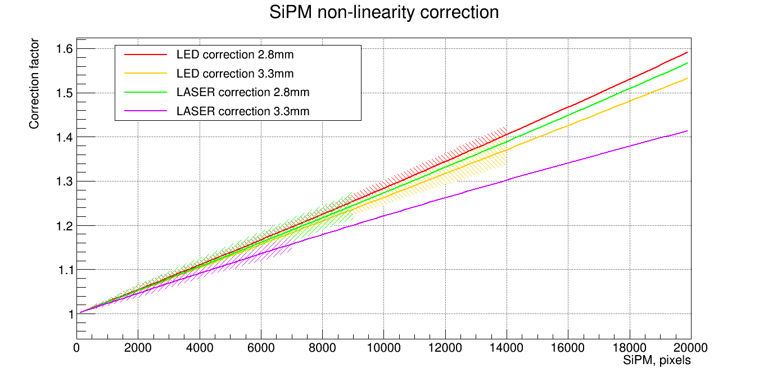
\includegraphics[width=\linewidth]{Figures/LaserNonLin.png}
\caption{Graph of the correction factor vs. number of pixels fired. The correction factor is the number the output needs to be multiplied by in order to obtain the linear output value. This means a perfectly linear device would always have a correction factor of 1. This data was obtained from shining a laser directly on the SiPM.}
\label{fig:NonLin}
\end{figure}

\begin{figure}
\centering
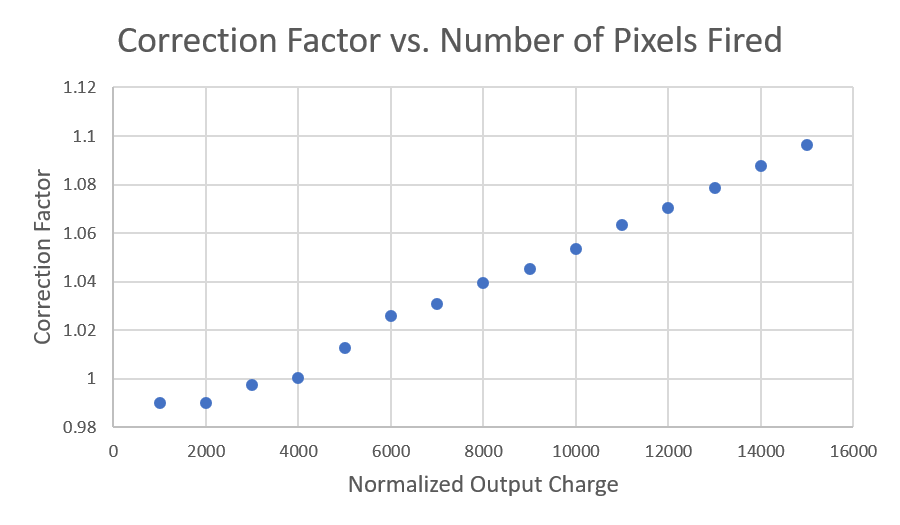
\includegraphics[width=\linewidth]{Figures/CorFac.png}
\caption{Graph of the correction factor vs. number of pixels fired. The correction factor is the number the output needs to be multiplied by in order to obtain the linear output value. This means a perfectly linear device would always have a correction factor of 1. This data was obtained from the SiPM simulation.}
\label{fig:Cor}
\end{figure}

Using the simulation we can also look at the pulse shape of the SiPM. This pulse shape should theoretically be the same obtained from test beam data. One of the main things that is necessary to look at is does the pulse shape change significantly with a change in input energy. As shown is figure~\ref{fig:SimPul} does not significantly change with different energies.

\begin{figure}
\centering
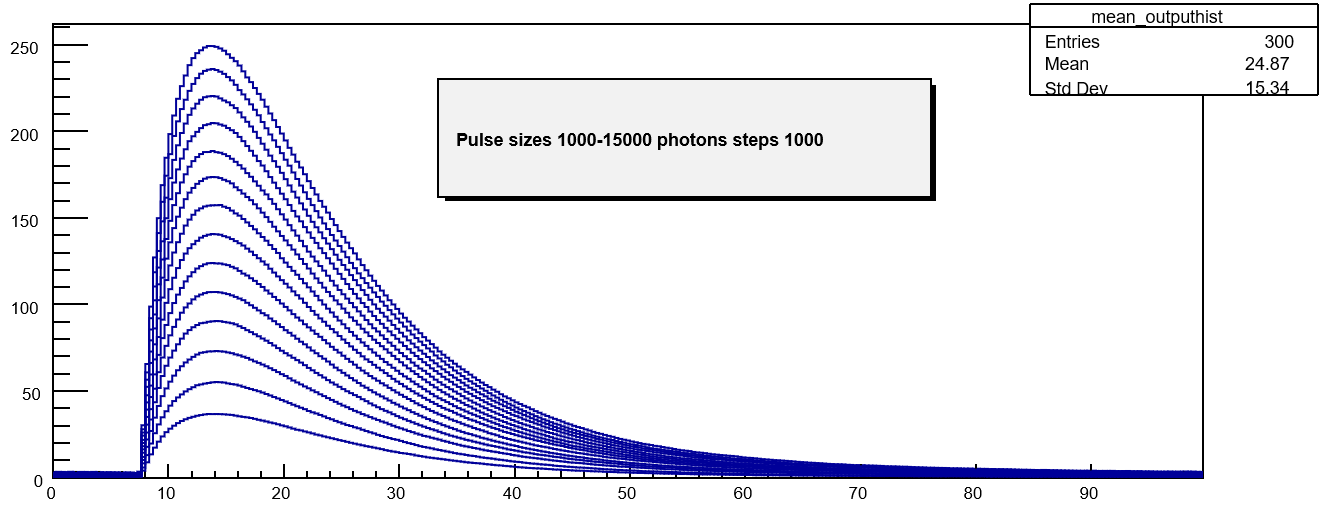
\includegraphics[width=\linewidth]{Figures/SimPul.png}
\caption{Pulse shapes from the SiPM simulation. They are stacked on top of each other to highlight any differences from an increase input photon count.}
\label{fig:SimPul}
\end{figure}

One effect of the saturation that is less understood and harder to implement is that the pixels can sometimes recharge faster. This effect is due to the QIE chips in the readout modules which in addition to taking and processing the charge from the SiPMs also supply the charge that recharges the capacitors for each individual pixel. The capacitors for the pixels recharge exponentially just like normal RC circuits. Normally the time constant for the capacitors is about 9ns which means the capacitor is basically completely charges after 20ns but this is when the SiPM is outputting a very low amount of charge to the QIE chips. When the SiPM is outputting more charge the QIE chips then supply more charge to the SiPM recharging the pixels faster. When the pixels recharge fast they will fire off closer to their maximum charge even when hit in rapid succession. This means as saturation becomes more prevalent with a high number of incident photons this reduces the effects of saturation. The effect of different recharge time for the pixels can be see in figure~\ref{fig:trc}.

\begin{figure}
\centering
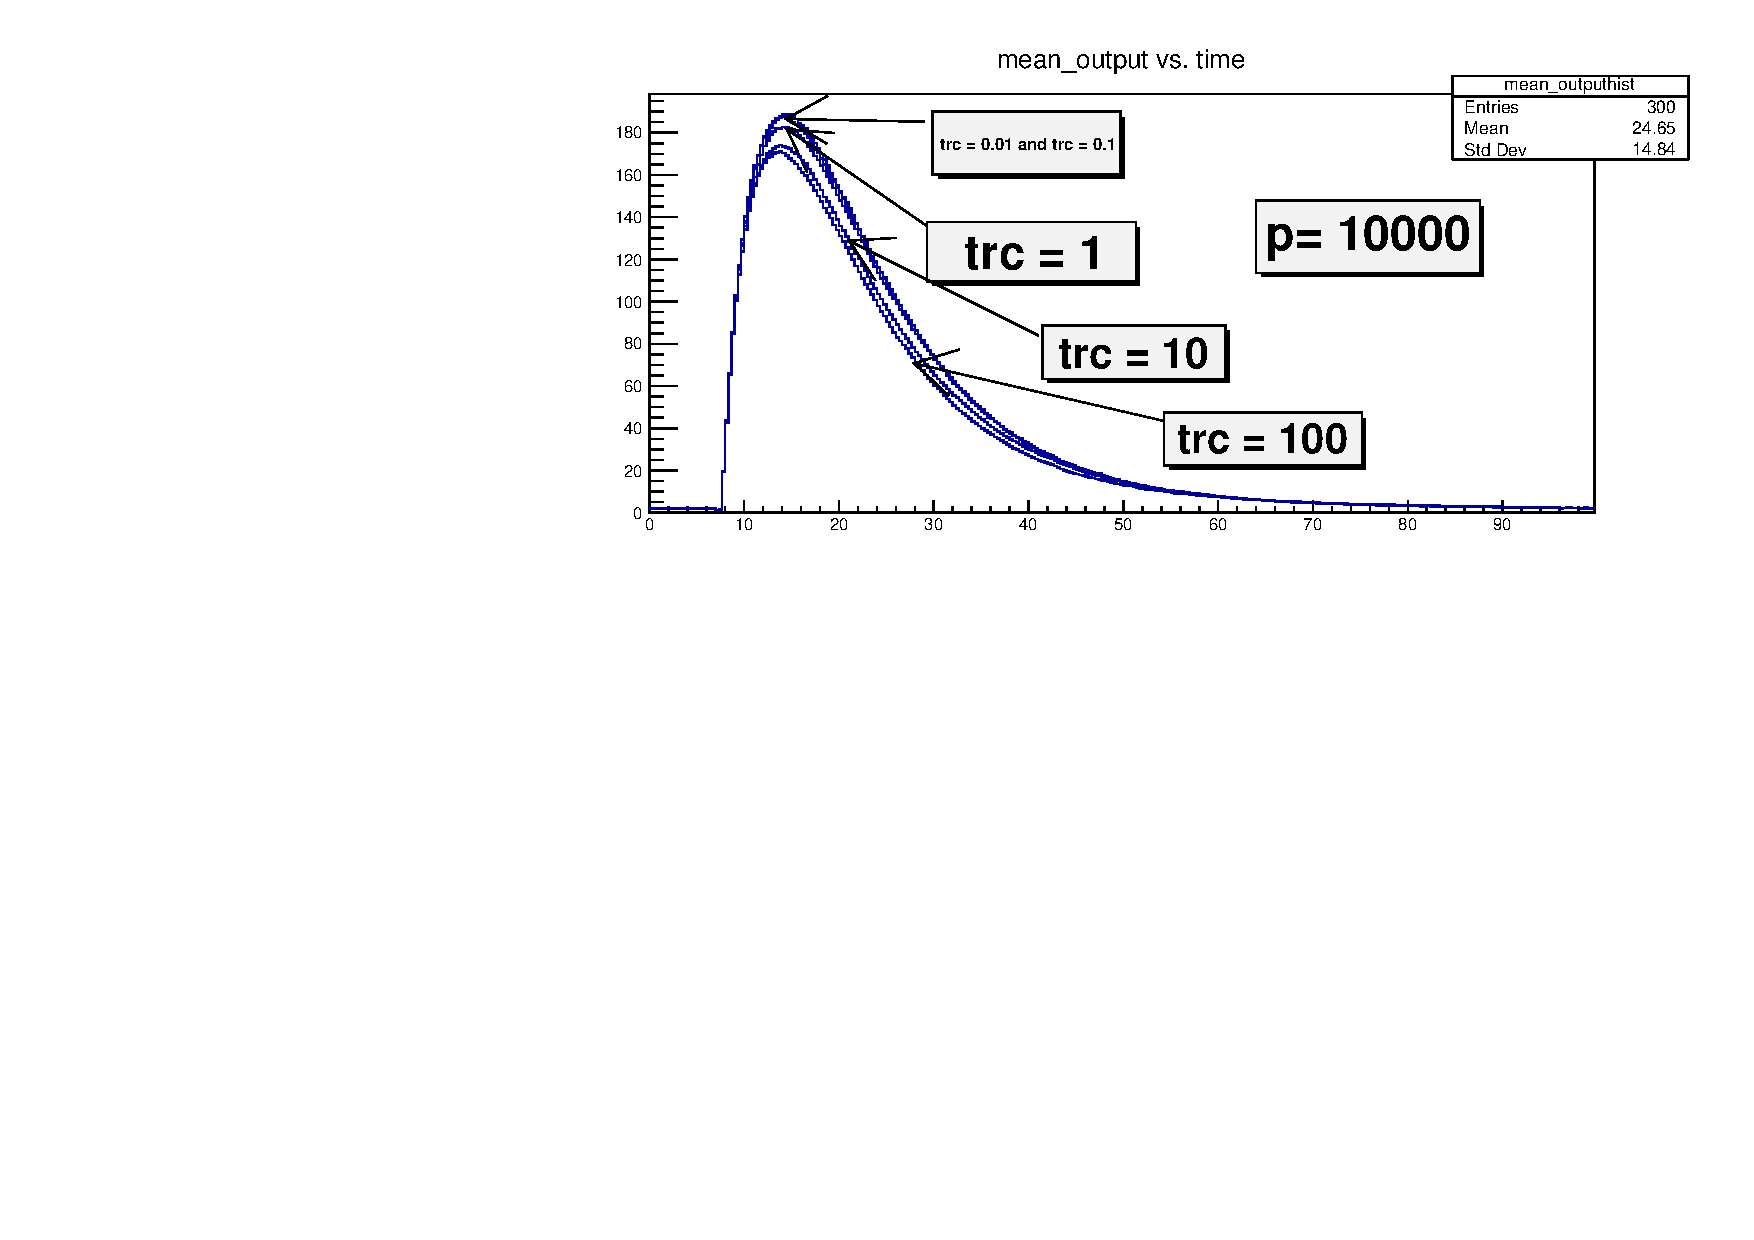
\includegraphics[width=\linewidth]{Figures/p10000trc.pdf}
\caption{Output pulses of the SiPM simulation with 10000 incidents photons comparing the effect of changing the recharge time constant on the pixels. The TRC value is the recharge time constant.}
\label{fig:trc}
\end{figure}

We can compare the pulse shape from the simulation to the one obtained from test beam data. Theoretically these pulses should be the same. For comparison we simply plot the two pulse shapes on top of each other and see if there are any major differences. To minimize the interference of other effects like non-linearity we can compare pulses from similar output charge. Using the conversion ratio of 40 fC to 1 photo electron we can compare pulses from the same charge range. For instance, for the charge range 10,000-29,000 fC we compare it a pulse of 500 photo electrons from the simulation. Figures ~\ref{fig:1comparison_together}-~\ref{fig:3comparison_together} show these comparisons. While they do have the same basic shape there are some significant differences mostly the simulation is much narrower in the base.

\begin{figure}
\centering
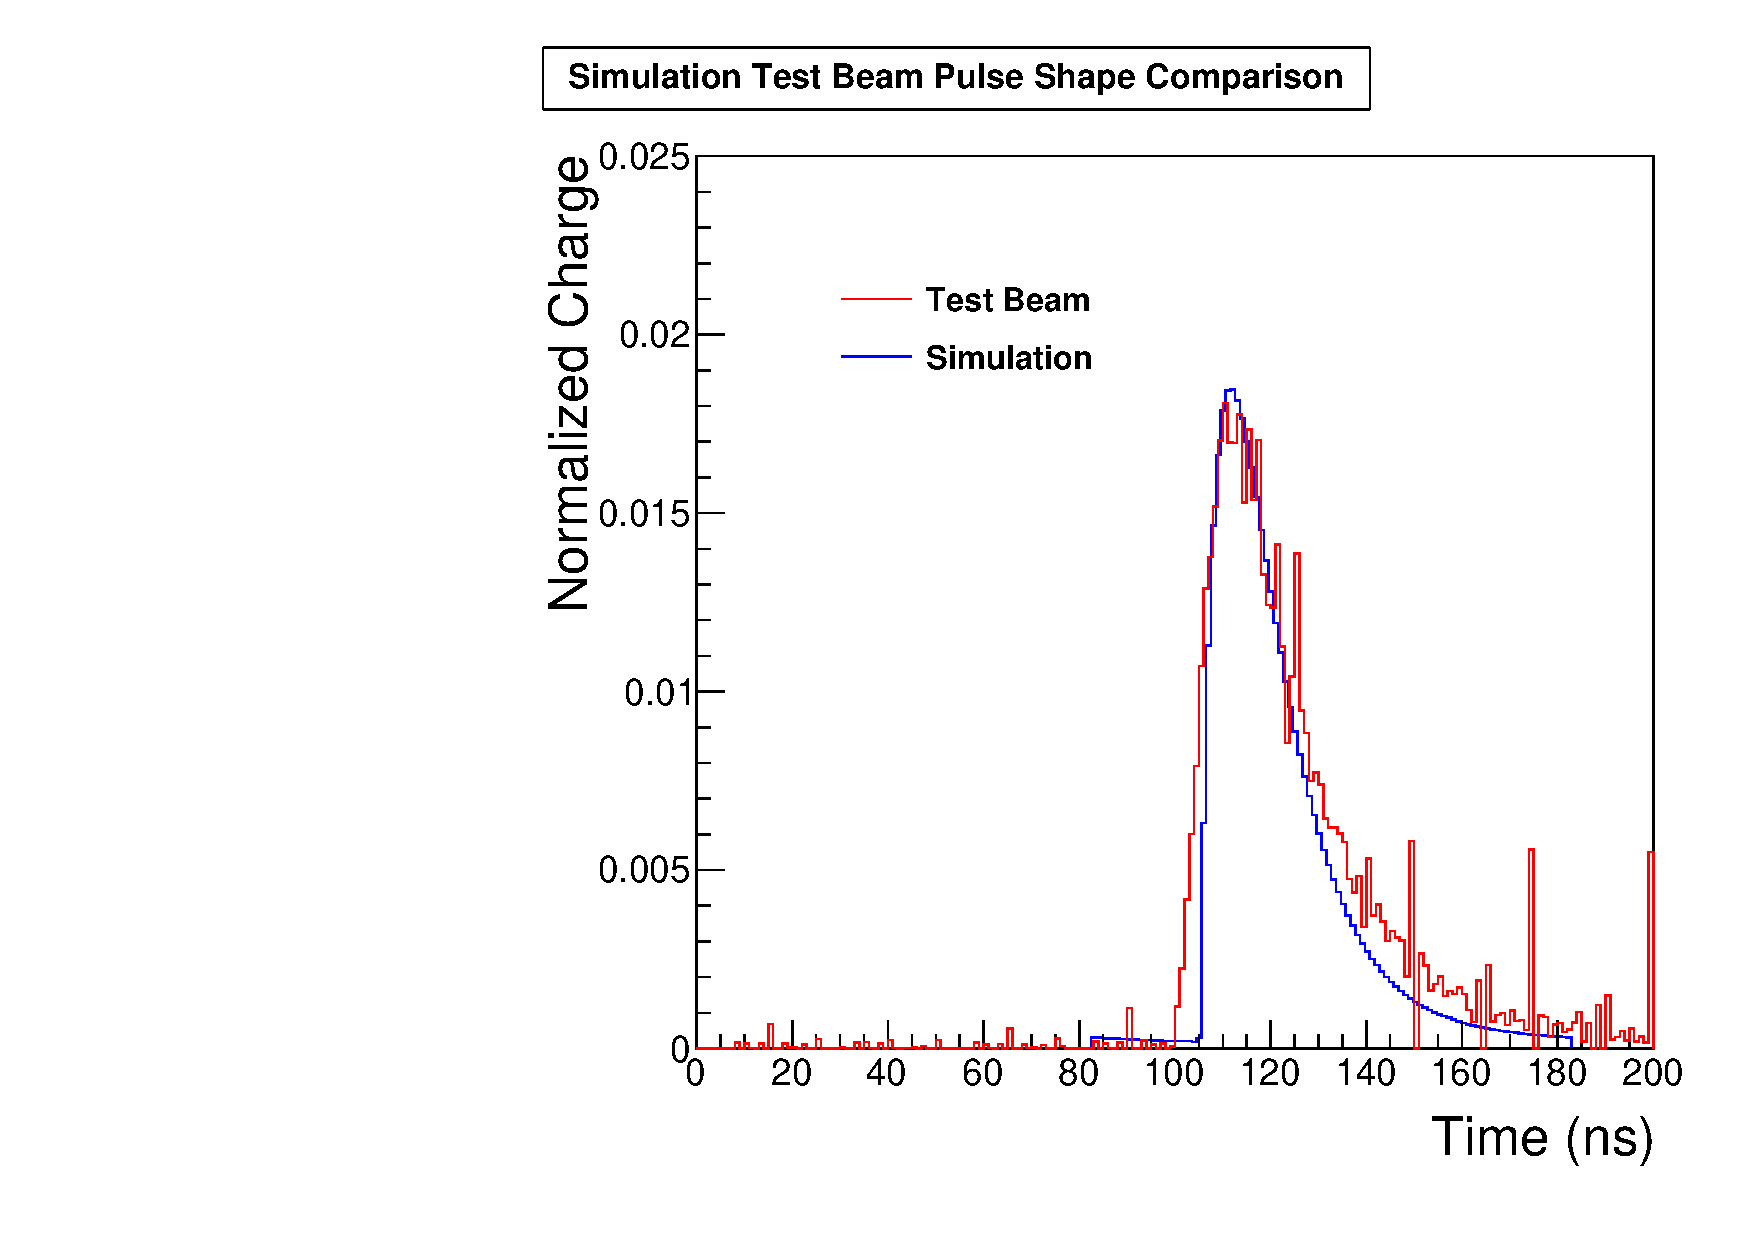
\includegraphics[width=0.495\linewidth]{Figures/10Comparison.pdf}
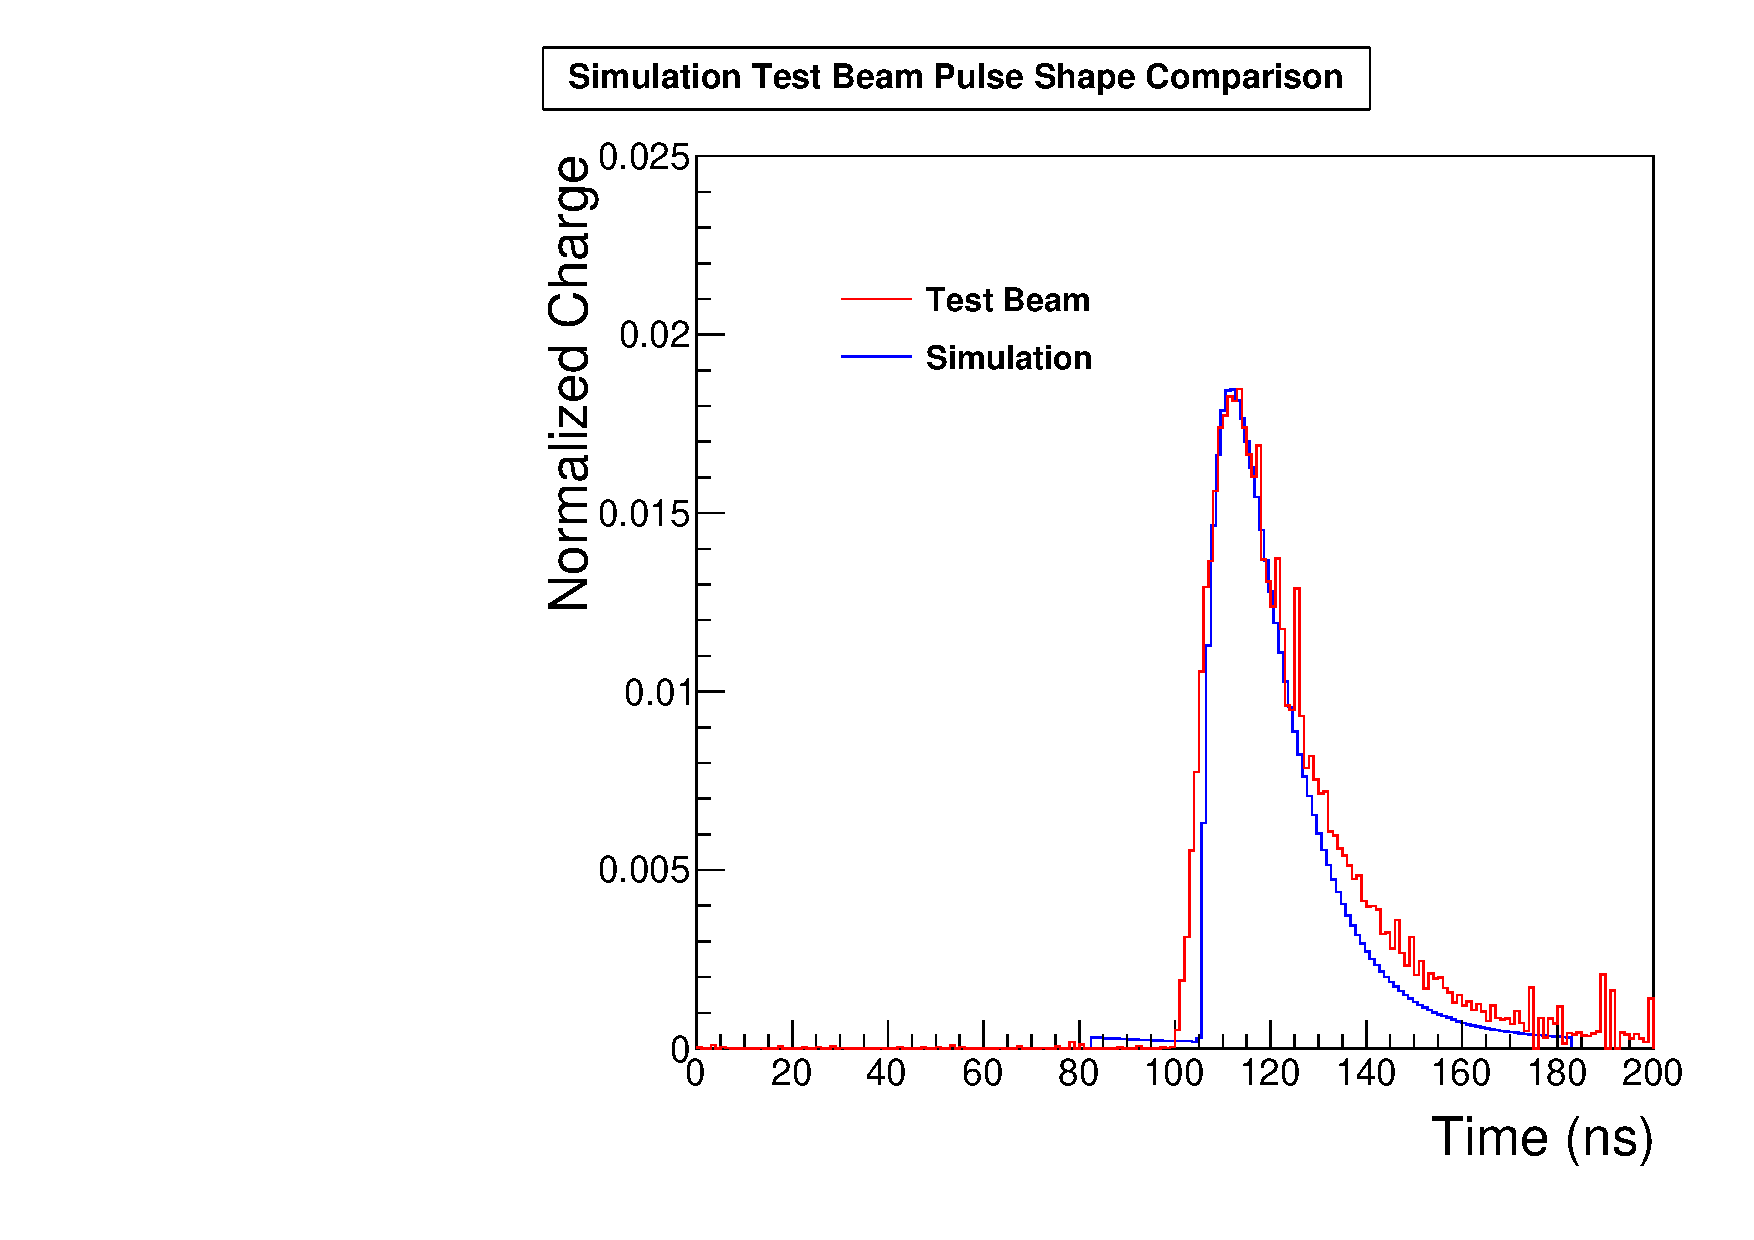
\includegraphics[width=0.495\linewidth]{Figures/29Comparison.pdf}
\caption{Histogram of the pulse shapes from the simulation and the test beam overlapping for comparison purposes. On the left the charge range is 10,000-29,000 fC on the right is 29,000-50,000 fC}
\label{fig:1comparison_together}
\end{figure}

\begin{figure}
\centering
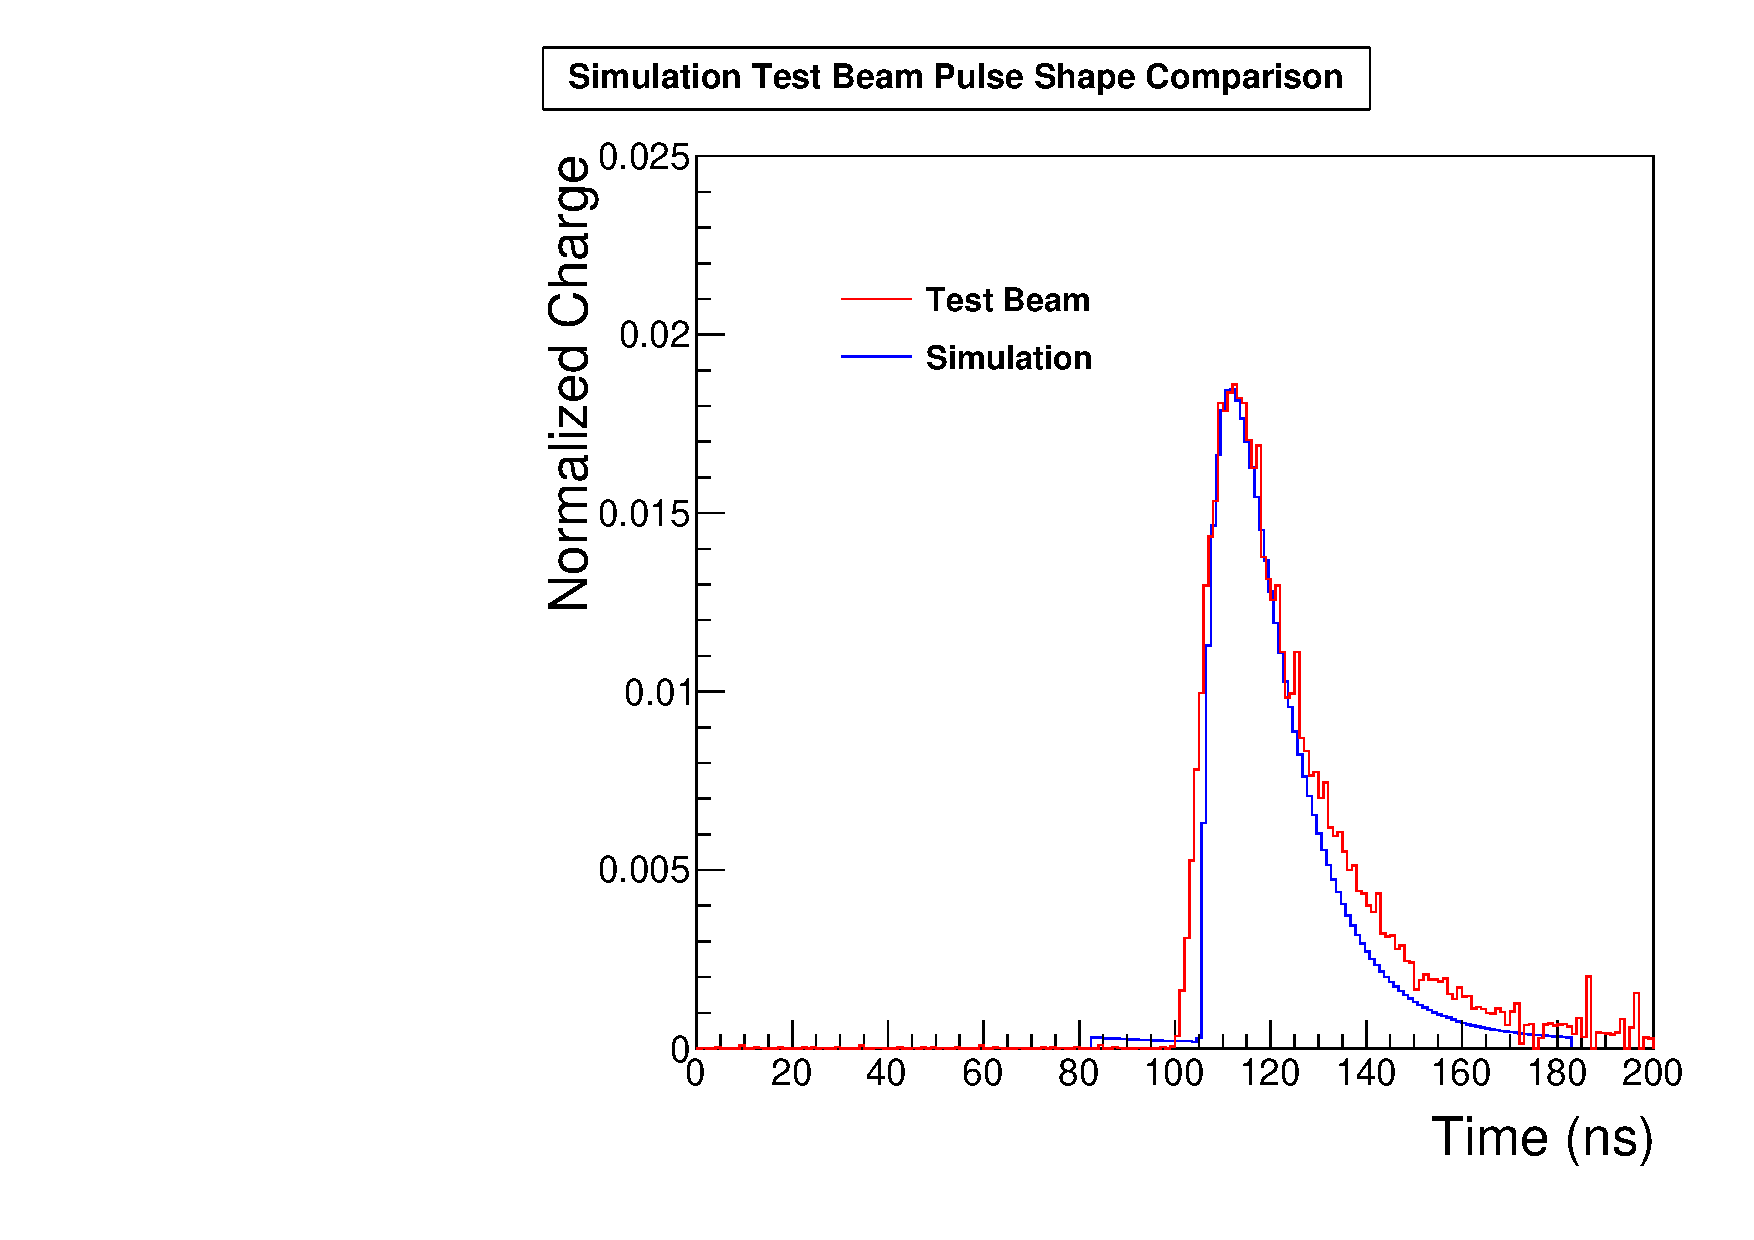
\includegraphics[width=0.495\linewidth]{Figures/50Comparison.pdf}
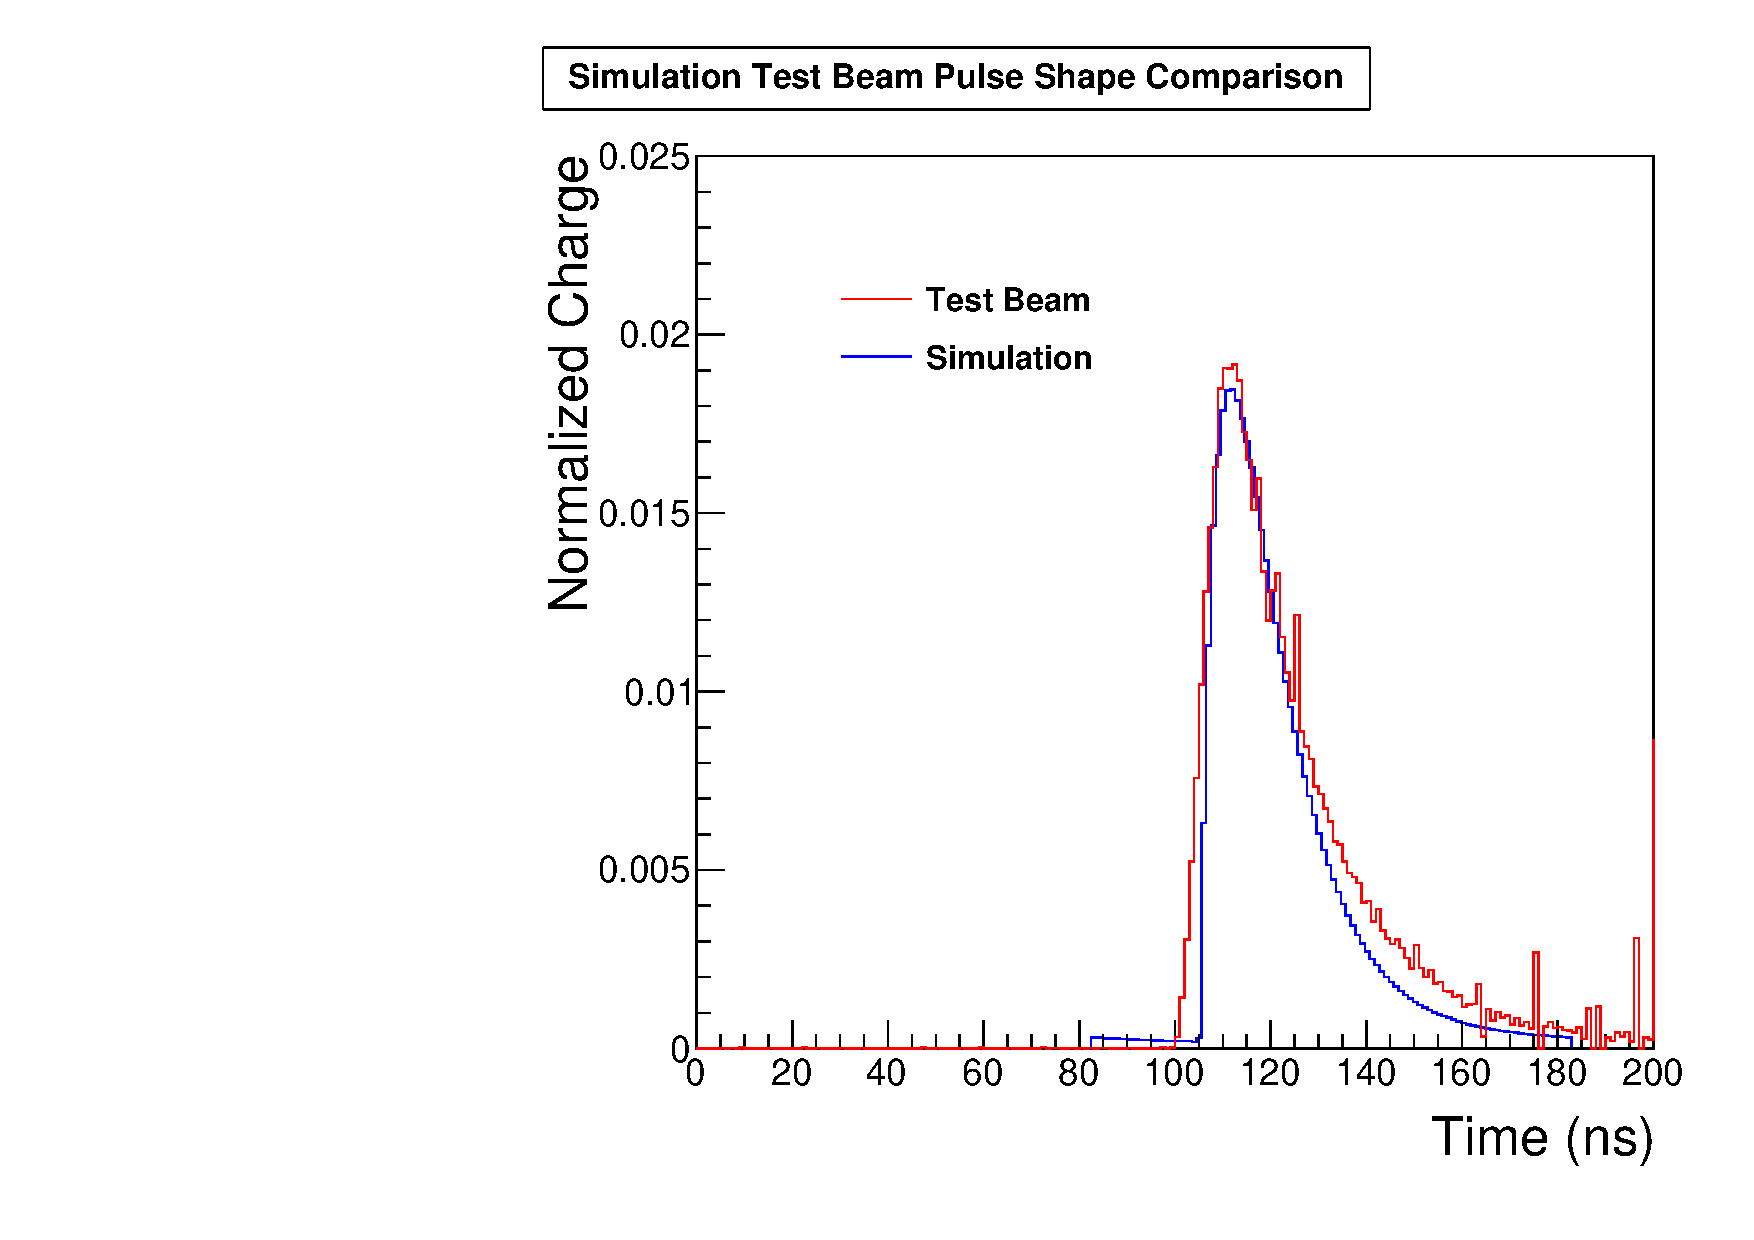
\includegraphics[width=0.495\linewidth]{Figures/80Comparison.pdf}
\caption{Histogram of the pulse shapes from the simulation and the test beam overlapping for comparison purposes. On the left the charge range is 50,000-80,000 fC on the right is 80,000-125,000 fC}
\label{fig:2comparison_together}
\end{figure}

\begin{figure}
\centering
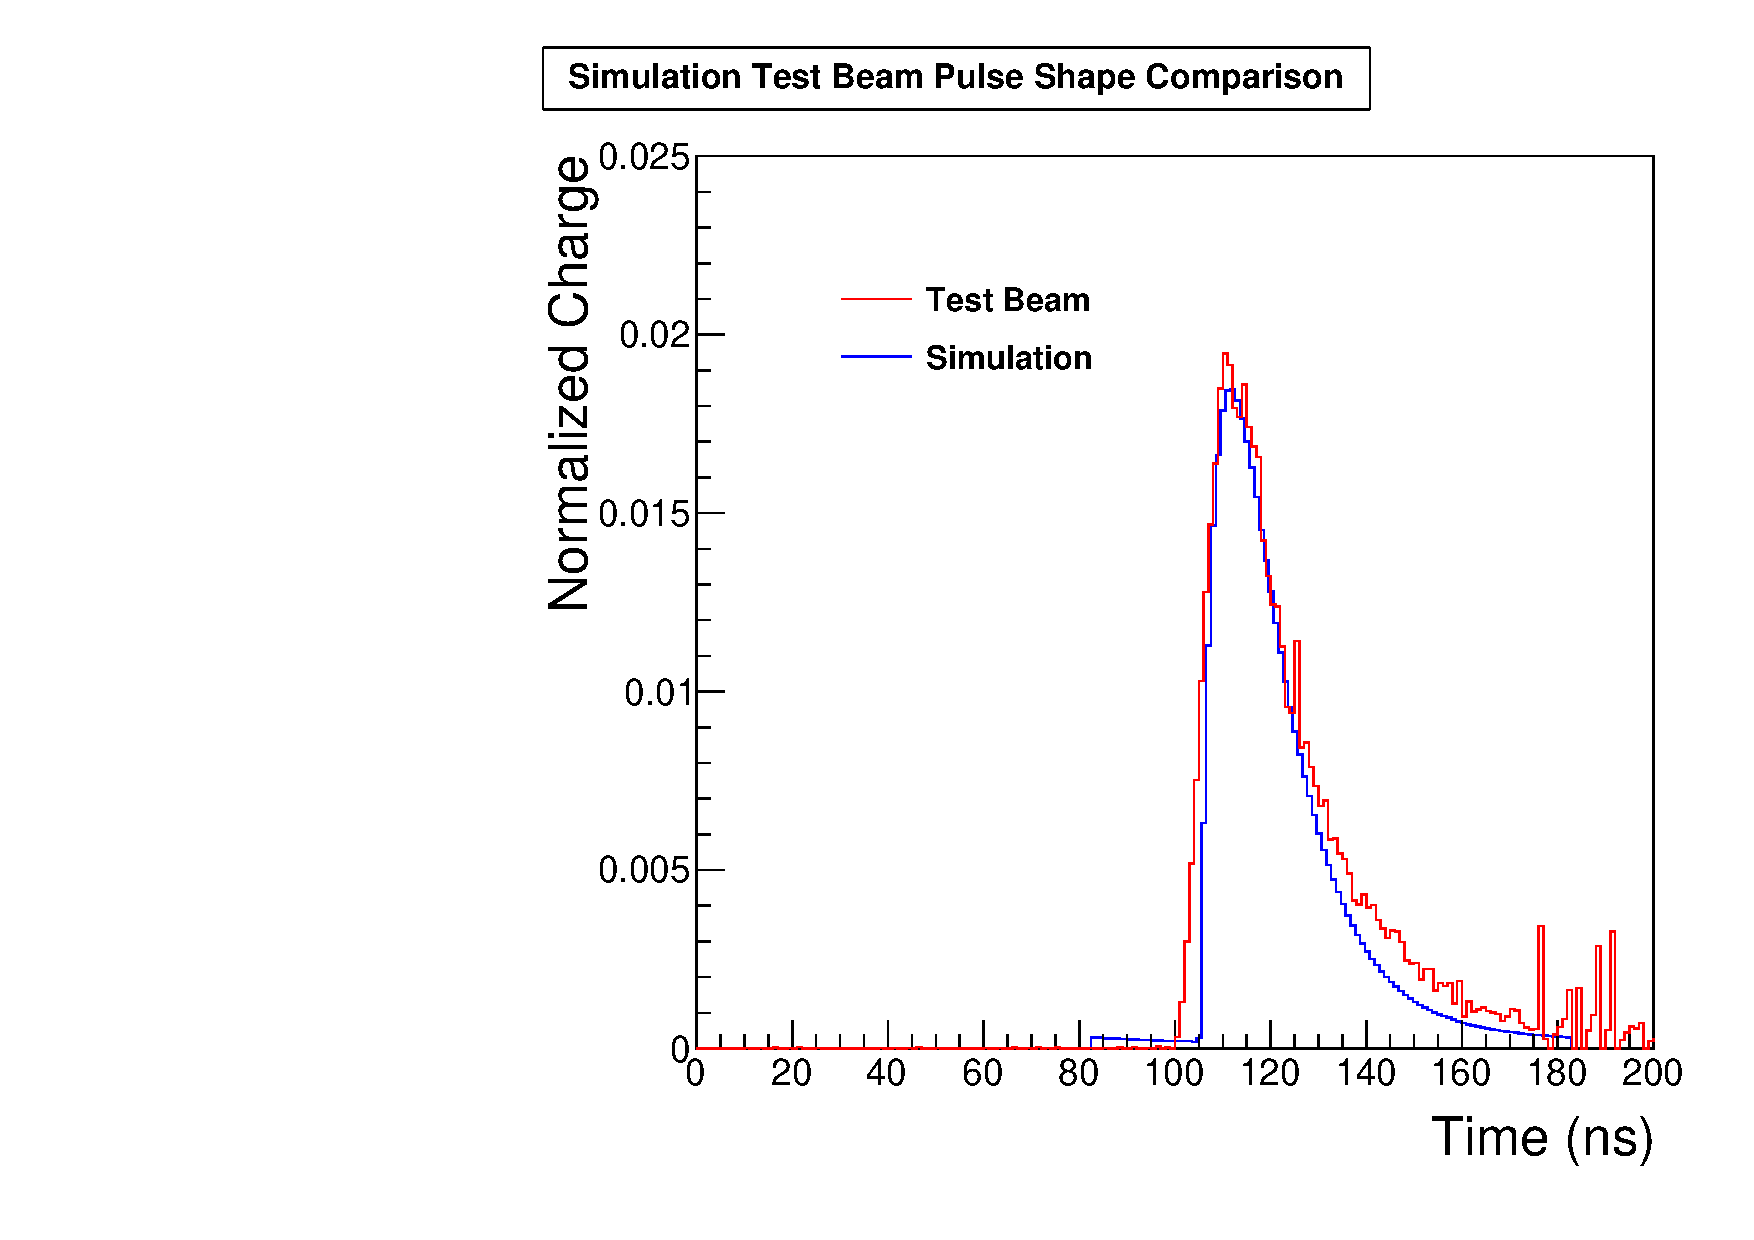
\includegraphics[width=0.495\linewidth]{Figures/125Comparison.pdf}
\caption{Histogram of the pulse shapes from the simulation and the test beam overlapping for comparison purposes. On the left the charge range is 10,000-29,000 fC on the right is 125,000-168,000 fC}
\label{fig:3comparison_together}
\end{figure}

\section{Conclusions}

